\chapter{Análise dos dados}\label{cap:analise-dos-dados}

A análise dos dados é essencial para o estudo. A partir da análise é que 
será possível determinar se o servidor HTTP objeto do estudo, o Nginx é mais 
eficiente do que o Apache. Os dados utilizados nessa análise são a média dos 
quatro testes realizados para cada quantidade total de requisições, 
correspondentes as porcentagens de requisições feitas de forma simultânea.

A análise será feita a partir da construção de gráficos comparativos e análise 
dos dados brutos coletados nos testes, observando a média 
entre os quinze valores coletados de acordo com a quantidade de requisições e 
dentro de cada faixa de valores para requisições. As faixas de valores de 
requisição estão expostas a seguir.

\section{Organização dos gráficos e dados}

Para melhor analisar o comportamento dos servidores em cada métrica, foram 
gerados quatro gráficos: três separados em faixas de valores de acordo com a 
quantidade total de requisições e um gráfico com todos os valores 
de requisições. As faixas são:

\begin{itemize}
	\item \textbf{Faixa 1} - Entre 1.000 e 5.000 requisições totais;
	\item \textbf{Faixa 2} - Entre 6.000 e 10.000 requisições totais;
	\item \textbf{Faixa 3} - Entre 11.000 e 15.000 requisições totais;
\end{itemize}

Dispondo os gráficos dessa forma, é possível analisar os dados de acordo com 
a quantidade de usuários utilizando o sistema e analisar o comportamento dos 
servidores HTTP de uma forma geral.

\section{Gráficos}
Todos os gráficos foram gerados usando a ferramenta de geração de gráfico do 
\citeonline{LOcalc}.
\subsection{Média do Tempo Total de Execução Dos Testes}
\subsubsection{Faixa 1}

blabla
\begin{figure}[htb]
	\centering
	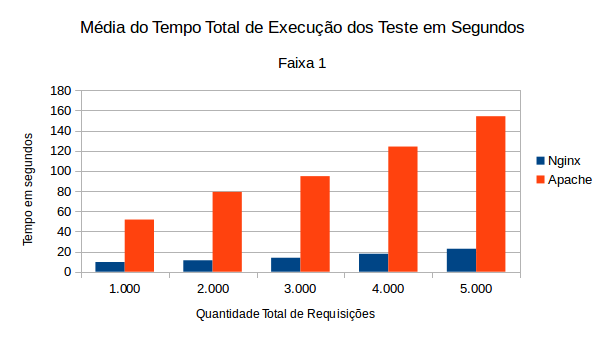
\includegraphics[width=0.6\linewidth]{graficos/grafico1-f1} 
	\caption{Média do Tempo Total de Execução dos Testes - Faixa 1}
	\label{fig:grafico1-f1}
\end{figure}

blabla

\subsubsection{Faixa 2}
blabla

\begin{figure}[htb]
	\centering
	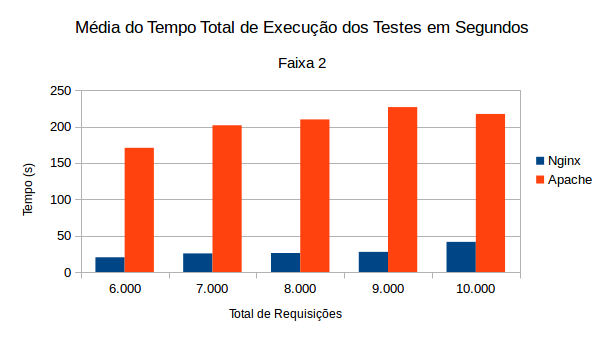
\includegraphics[width=0.6\linewidth]{graficos/grafico1-f2} 
	\caption{Média do Tempo Total de Execução dos Testes - Faixa 2}
	\label{fig:grafico1-f2}
\end{figure}
blabla

\subsubsection{Faixa 3}
blabla

\begin{figure}[htb]
	\centering
	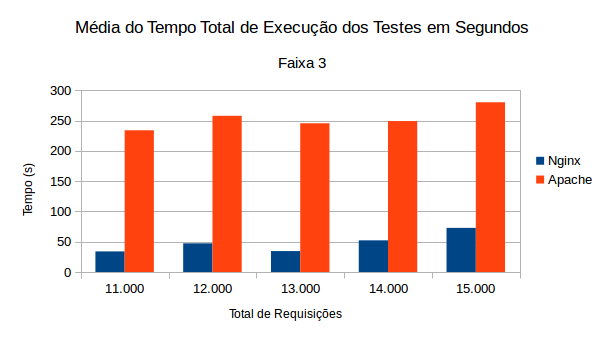
\includegraphics[width=0.6\linewidth]{graficos/grafico1-f3} 
	\caption{Média do Tempo Total de Execução dos Testes - Faixa 3}
	\label{fig:grafico1-f3}
\end{figure}
blabla


\subsection{Média da Quantidade Total de Dados Transmitidos}
\subsubsection{Faixa 1}

blabla
\begin{figure}[htb]
	\centering
	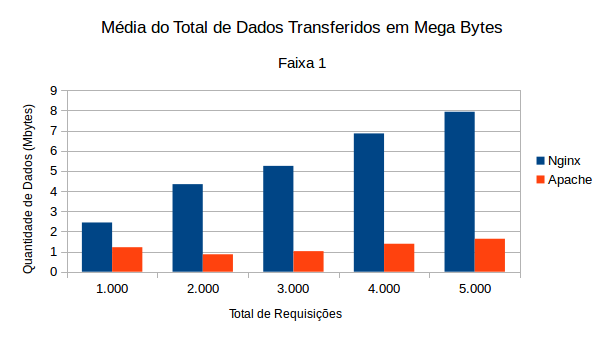
\includegraphics[width=0.6\linewidth]{graficos/grafico2-f1} 
	\caption{Média do Total de Dados Transferidos - Faixa 1}
	\label{fig:grafico2-f1}
\end{figure}

blabla

\subsubsection{Faixa 2}
blabla

\begin{figure}[htb]
	\centering
	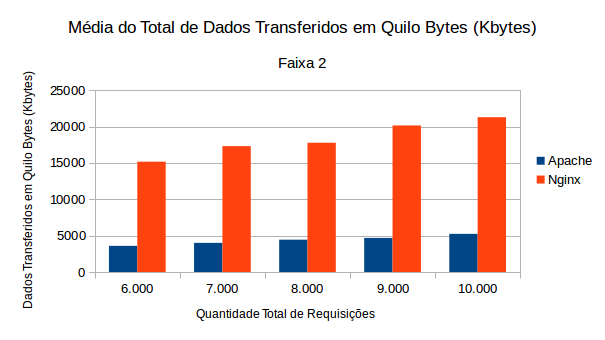
\includegraphics[width=0.6\linewidth]{graficos/grafico2-f2} 
	\caption{Média do Total de Dados Transferidos - Faixa 2}
	\label{fig:grafico2-f2}
\end{figure}
blabla

\subsubsection{Faixa 3}
blabla

\begin{figure}[htb]
	\centering
	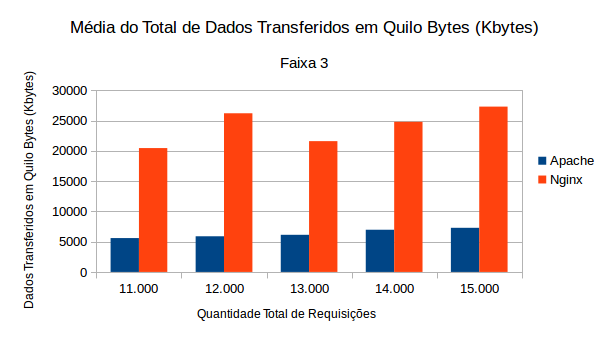
\includegraphics[width=0.6\linewidth]{graficos/grafico2-f3} 
	\caption{Média do Total de Dados Transferidos - Faixa 3}
	\label{fig:grafico2-f3}
\end{figure}
blabla

\subsection{Média da Quantidade de Texto HTML Transmitido}
\subsubsection{Faixa 1}

blabla
\begin{figure}[htb]
	\centering
	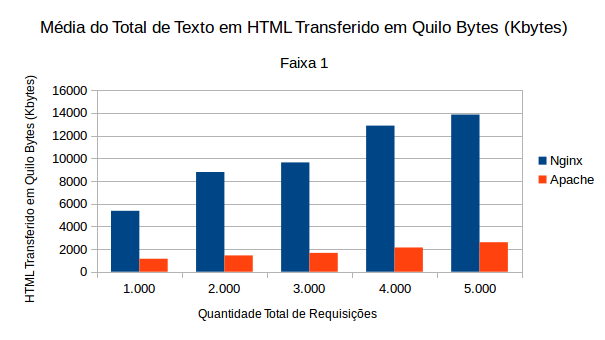
\includegraphics[width=0.6\linewidth]{graficos/grafico3-f1} 
	\caption{Média do Total de Texto em HTML Transferido - Faixa 1}
	\label{fig:grafico3-f1}
\end{figure}

blabla

\subsubsection{Faixa 2}
blabla

\begin{figure}[htb]
	\centering
	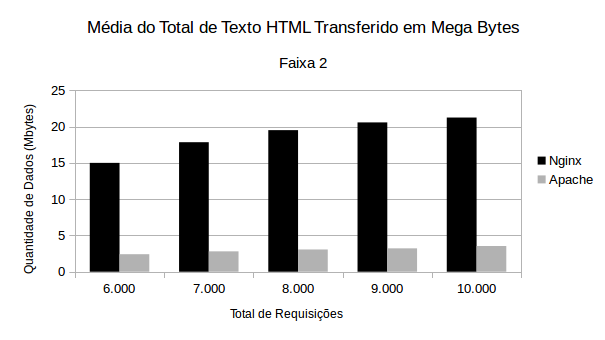
\includegraphics[width=0.6\linewidth]{graficos/grafico3-f2} 
	\caption{Média do Total de Texto em HTML Transferido - Faixa 2}
	\label{fig:grafico3-f2}
\end{figure}
blabla

\subsubsection{Faixa 3}
blabla

\begin{figure}[htb]
	\centering
	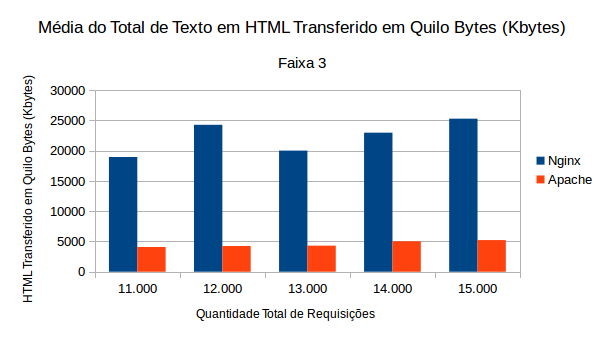
\includegraphics[width=0.6\linewidth]{graficos/grafico3-f3} 
	\caption{Média do Total de Texto em HTML Transferido - Faixa 3}
	\label{fig:grafico3-f3}
\end{figure}
blabla

%\section{Análise}\label{sec:analise-dos-dados}
